\section {Traitement des informations}



\subsection*{Cockburn du traitement des informations}

Le cas d'utilisation \textit{Process} concerne le traitement des informations. Cette étape se place en seconde position dans l'ordre des étapes de la méthode GTD. La description textuelle selon le canevas CockBurn est présentée ci-dessous :

\begin{center}
\begin{tabular}{|p{1.1in}|p{0.6in}|p{1.8in}|p{1.5in}|} \hline 
\textbf{Cas d'utilisation} & \multicolumn{3}{|p{2.9in}|}{Traiter les informations} \\ \hline 
\textbf{Acteur} & \multicolumn{3}{|p{2.9in}|}{Utilisateur} \\ \hline 
\textbf{Parties 
prenantes et intérêts} & \multicolumn{3}{|p{2.9in}|}{Une fois la collecte des informations 
faîte, on détermine si des tâches pertinentes en résultent.} \\ \hline 
\textbf{Niveau} & \multicolumn{3}{|p{2.9in}|}{Objectif utilisateur} \\ \hline 
\textbf{Portée} & \multicolumn{3}{|p{2.9in}|}{~} \\ \hline 
\textbf{Pré-conditions} & \multicolumn{3}{|p{2.9in}|}{L'utilisateur a procédé à la collecte 
des informations} \\ \hline 
\textbf{Post-conditions} & \multicolumn{3}{|p{2.9in}|}{Les informations ont été traitées, 
de nouvelles tâches ont été créées si besoin} \\ \hline 



\textbf{Scénario nominal} & \textbf{Etapes}  & \multicolumn{2}{|p{2.5in}|}{\textbf{Action}}   \\ \hline 
 & 1 & \multicolumn{2}{|p{2.5in}|}{L'information nécessite une action} \\ \hline 
 & 2 & \multicolumn{2}{|p{2.5in}|}{La 
tâche ne peut pas être faite immédiatement} \\ \hline 
 & 3 & \multicolumn{2}{|p{2.5in}|}{Création d'une tâche} \\ \hline 
\textbf{Contraintes} & \textbf{Type} & \multicolumn{2}{|p{2.5in}|}{\textbf{Description}} \\ \hline 
 & ~ & \multicolumn{2}{|p{2.5in}|}{~} \\ \hline 
\textbf{Priorité} & \multicolumn{3}{|p{2.9in}|}{Très élevée (5/5)} \\ \hline 
\textbf{Performance} & \multicolumn{3}{|p{2.9in}|}{~} \\ \hline 
\textbf{Fréquences} & \multicolumn{3}{|p{2.9in}|}{Dès que l'utilisateur collecte de nouvelles 
informations, il doit les traiter.} \\ \hline 
\end{tabular}\end{center}





\subsection*{Scenario du traitement des informations}

Ce scénario complète le cas d'utilisation décrit précédemment. Il présente les interactions entre l'utilisateur et le système dans le cas où l'utilisateur a recueilli toutes les informations susceptibles d'engendrer des actions.


	\begin{figure}[H]
	\begin{center}
	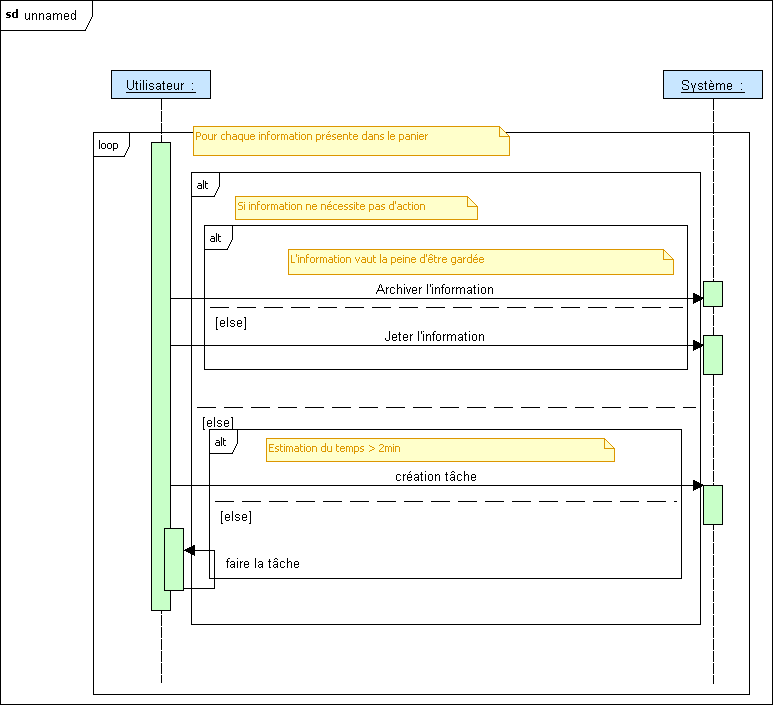
\includegraphics[scale=0.5]{diagrams/scenario_traitement.png}
	\caption{Diagramme UML  - Scénario traitement des données}
	\end{center}
	\end{figure}
	
	\bigskip

\subsection*{Diagramme d'objets} 

Afin d'observer l'impact du cas d'utilisation Traitement des informations sur les objets, voici deux diagrammes d'objets représentant leurs états avant et après le traitement.

	\subsubsection{Avant le traitement des données}
	
	\begin{figure}[H]
	\begin{center}
	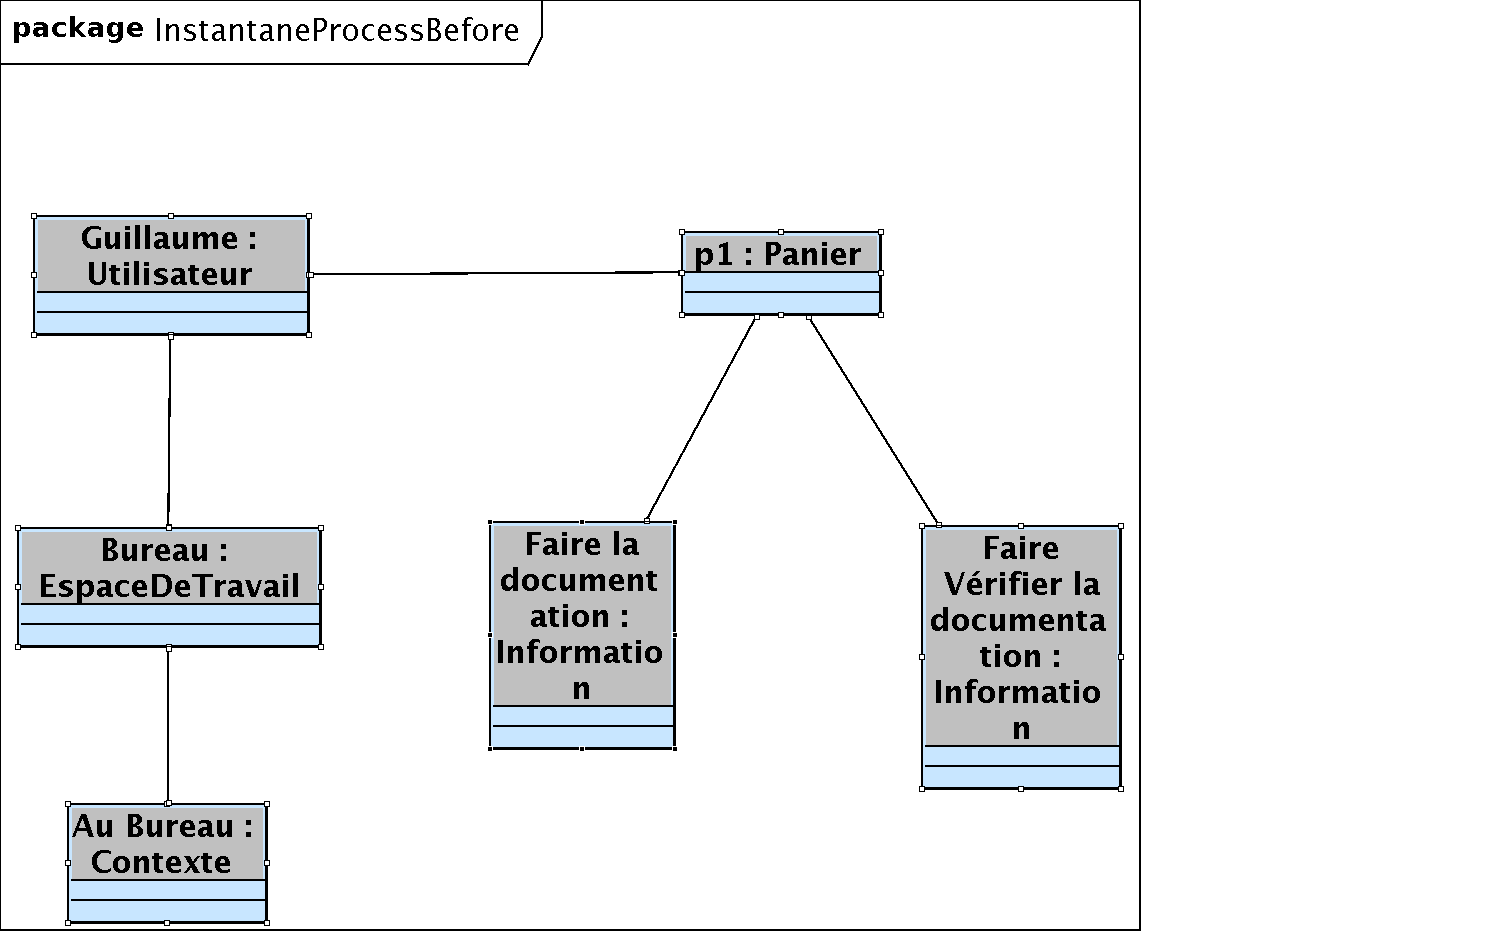
\includegraphics[scale=0.3]{diagrams/diag_objets_process_before.png}
	\caption{Diagramme d'objets UML  - Avant le traitement des informations}
	\end{center}
	\end{figure}
	
	\bigskip
	
	L'utilisateur a procédé à la collecte des différentes informations nécessitant une intervention de l'utilisateur, elles peuvent toutes potentiellement devenir des tâches. Elles sont associées au panier de l'utilisateur. Ce dernier se trouve dans un espace de travail particulier nommé Bureau.
	
	\subsubsection{Après le traitement des données}
	
	\begin{figure}[H]
	\begin{center}
	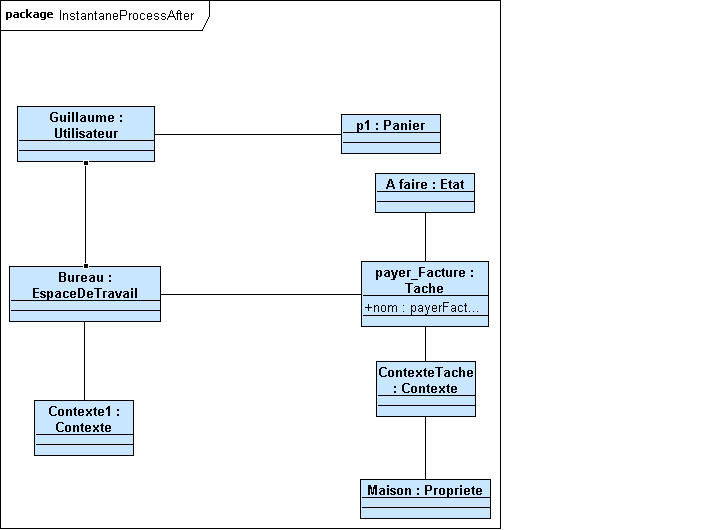
\includegraphics[scale=0.5]{diagrams/diag_objets_process_after.png}
	\caption{Diagramme d'objets UML  - Après le traitement des informations}
	\end{center}
	\end{figure}
	
	\bigskip 
	
	
	L'utilisateur procède au traitement des données : celu-ci consiste à définir si une information nécessite de devenir une tâche à effectuer. Dans le cas présent, l'information 1 entraîne la création de la tâche Payer\_facture. Cette dernière est forcément associée à un contexte.  